\documentclass{article}
\usepackage{amsmath}
\usepackage{amsfonts}
\usepackage{amssymb}
\usepackage{tikz}
\usetikzlibrary{positioning}

\title{HyperionDev - Tuorial - Neural Networks}

\begin{document}
	\maketitle
	
	\section*{Overview}
	
	This document describes a simple feedforward neural network with bias terms included. It covers the architecture of the neural network, forward pass computations, backward pass computations, regularisation techniques, and weight updates. 

Although there are multiple libraries like TensorFlow, Keras, PyTorch, and Scikit-Learn, it is important to know the way, under the hood of how a neural network is trained. 

This will allow you to at least describe it, understand it and eventually debug it if need be. 

You should also be able to understand all the moving parts here, like the parameters involved: \textit{learning rate}, \textit{initialiser}, \textit{regularisation} ... Most of the libraries have default parameters that may not suit your work. You must know what you are changing and how it affects training in a Machine Learning environment.
	
	\newpage
	
	\section*{Neural Network Diagram}
	
	\begin{figure}[h!]
		\centering
		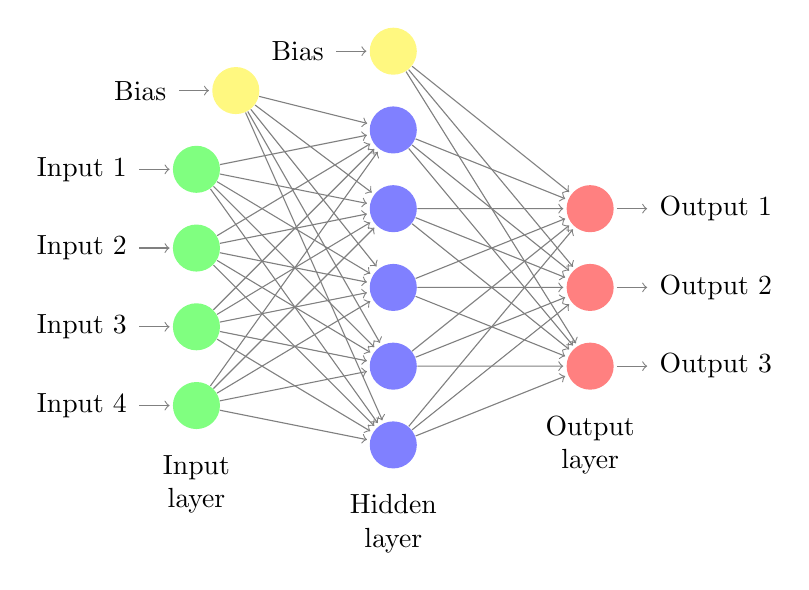
\begin{tikzpicture}[shorten >=1pt,->,draw=black!50, node distance=1.5cm]
			\tikzstyle{every pin edge}=[<-,shorten <=1pt]
			\tikzstyle{neuron}=[circle,fill=black!25,minimum size=17pt,inner sep=0pt]
			\tikzstyle{input neuron}=[neuron, fill=green!50];
			\tikzstyle{output neuron}=[neuron, fill=red!50];
			\tikzstyle{hidden neuron}=[neuron, fill=blue!50];
			\tikzstyle{bias neuron}=[neuron, fill=yellow!50];
			\tikzstyle{annot} = [text width=4em, text centered]
			
			% Define layer separation distance
			\def\layersep{2.5cm}
			
			% Draw the input layer nodes
			\foreach \name / \y in {1,...,4}
			\node[input neuron, pin=left:Input \y] (I-\name) at (0,-\y) {};
			
			% Draw the input layer bias node
			\node[bias neuron, pin=left:Bias] (I-bias) at (0.5,0) {};
			
			% Draw the hidden layer nodes
			\foreach \name / \y in {1,...,5}
			\path[yshift=0.5cm]
			node[hidden neuron] (H-\name) at (\layersep,-\y cm) {};
			
			% Draw the hidden layer bias node
			\node[bias neuron, pin=left:Bias] (H-bias) at (\layersep,0.5) {};
			
			% Draw the output layer nodes
			\foreach \name / \y in {1,...,3}
			\path[yshift=-0.5cm]
			node[output neuron, pin={[pin edge={->}]right:Output \y}] (O-\name) at (2*\layersep,-\y cm) {};
			
			% Connect every node in the input layer with every node in the hidden layer.
			\foreach \source in {1,...,4}
			\foreach \dest in {1,...,5}
			\path (I-\source) edge (H-\dest);
			
			% Connect the input bias node with every node in the hidden layer.
			\foreach \dest in {1,...,5}
			\path (I-bias) edge (H-\dest);
			
			% Connect every node in the hidden layer with every node in the output layer.
			\foreach \source in {1,...,5}
			\foreach \dest in {1,...,3}
			\path (H-\source) edge (O-\dest);
			
			% Connect the hidden bias node with every node in the output layer.
			\foreach \dest in {1,...,3}
			\path (H-bias) edge (O-\dest);
			
			% Annotate the layers
			\node[annot,below of=I-3, node distance=2cm] {Input layer};
			\node[annot,below of=H-3, node distance=3cm] {Hidden layer};
			\node[annot,below of=O-2, node distance=2cm] {Output layer};
		\end{tikzpicture}
		\caption{A simple feedforward neural network with one hidden layer. Bias nodes are shown in yellow.}
	\end{figure}
	
	\section*{Forward Pass}
	
	Given:
	\begin{itemize}
		\item Input data $\mathbf{X}$ of shape $(m, n)$, where $m$ is the number of samples and $n$ is the number of input features.
		\item Weights and biases for the hidden layer: $\mathbf{W1}$ of shape $(n, h)$ and $\mathbf{b1}$ of shape $(1, h)$, where $h$ is the number of hidden units.
		\item Weights and biases for the output layer: $\mathbf{W2}$ of shape $(h, c)$ and $\mathbf{b2}$ of shape $(1, c)$, where $c$ is the number of classes.
	\end{itemize}
	
	1. Compute the input to the hidden layer:
	\[
	\mathbf{Z1} = \mathbf{X} \mathbf{W1} + \mathbf{b1}
	\]
	
	2. Apply the sigmoid activation function to get the hidden layer activations:
	\[
	\mathbf{A1} = \sigma(\mathbf{Z1}) = \frac{1}{1 + e^{-\mathbf{Z1}}}
	\]
	
	3. Compute the input to the output layer:
	\[
	\mathbf{Z2} = \mathbf{A1} \mathbf{W2} + \mathbf{b2}
	\]
	
	4. Apply the softmax activation function to get the output layer activations (probabilities):
	\[
	\mathbf{A2} = \text{softmax}(\mathbf{Z2}) = \frac{e^{\mathbf{Z2}}}{\sum_{j} e^{\mathbf{Z2_j}}}
	\]
	
	\section*{Backward Pass}
	
	Given:
	\begin{itemize}
		\item The predicted outputs $\mathbf{A2}$ and the true labels $\mathbf{Y}$.
	\end{itemize}
	
	1. Compute the error at the output layer:
	\[
	\mathbf{dZ2} = \mathbf{A2} - \mathbf{Y}
	\]
	
	2. Compute the gradient for the output layer weights $\mathbf{W2}$:
	\[
	\mathbf{dW2} = \frac{1}{m} \mathbf{A1}^T \mathbf{dZ2}
	\]
	
	3. Compute the gradient for the output layer biases $\mathbf{b2}$:
	\[
	\mathbf{db2} = \frac{1}{m} \sum_{i=1}^{m} \mathbf{dZ2_i}
	\]
	
	4. Backpropagate the error to the hidden layer:
	\[
	\mathbf{dA1} = \mathbf{dZ2} \mathbf{W2}^T
	\]
	
	5. Compute the gradient of the sigmoid activation function:
	\[
	\sigma'(\mathbf{Z1}) = \mathbf{A1} \circ (1 - \mathbf{A1})
	\]
	
	6. Compute the error at the hidden layer:
	\[
	\mathbf{dZ1} = \mathbf{dA1} \circ \sigma'(\mathbf{Z1})
	\]
	where $\circ$ denotes the element-wise product (Hadamard product).
	
	7. Compute the gradient for the hidden layer weights $\mathbf{W1}$:
	\[
	\mathbf{dW1} = \frac{1}{m} \mathbf{X}^T \mathbf{dZ1}
	\]
	
	8. Compute the gradient for the hidden layer biases $\mathbf{b1}$:
	\[
	\mathbf{db1} = \frac{1}{m} \sum_{i=1}^{m} \mathbf{dZ1_i}
	\]
	
	\section*{Regularisation}
	
	\subsection*{L1 Regularisation}
	Add the derivative of the L1 regularisation term to the weight gradients:
	\[
	\mathbf{dW2} += \lambda \, \text{sign}(\mathbf{W2})
	\]
	\[
	\mathbf{dW1} += \lambda \, \text{sign}(\mathbf{W1})
	\]
	
	\subsection*{L2 Regularisation}
	Add the derivative of the L2 regularisation term to the weight gradients:
	\[
	\mathbf{dW2} += \lambda \mathbf{W2}
	\]
	\[
	\mathbf{dW1} += \lambda \mathbf{W1}
	\]
	
	\section*{Weight Updates}
	
	Update the weights and biases using gradient descent:
	
	1. Update weights and biases for the hidden layer:
	\[
	\mathbf{W1} -= \alpha \mathbf{dW1}
	\]
	\[
	\mathbf{b1} -= \alpha \mathbf{db1}
	\]
	
	2. Update weights and biases for the output layer:
	\[
	\mathbf{W2} -= \alpha \mathbf{dW2}
	\]
	\[
	\mathbf{b2} -= \alpha \mathbf{db2}
	\]
	
\end{document}
